\documentclass[11pt]{article}

\usepackage{amsmath,amssymb,amsthm}
\usepackage{booktabs}
\usepackage{graphicx}
\usepackage[margin=1in]{geometry}
\usepackage{caption}
\usepackage{float}
\usepackage{placeins}
\usepackage{hyperref}
\hypersetup{hidelinks, bookmarksnumbered=true}

\graphicspath{{figs/}}
\captionsetup{font=small, skip=6pt, justification=raggedright}

\title{KPP Front-Speed Experiments (Sections 4.3 and 4.4)}
\author{KPP reproduction group}
\date{\today}

\begin{document}
\maketitle

\setcounter{section}{4}
\setcounter{subsection}{2}
\setcounter{figure}{4}

This excerpt reports the Kolmogorov--Petrovsky--Piskunov (KPP) experiments
from Shen et al.\ (arXiv:2601.20024v1). Section~4.3 treats a
two-dimensional cellular flow on \(\mathbb{T}^2\). Section~4.4 treats a
three-dimensional time-dependent Kolmogorov flow on \(\mathbb{T}^3\).
The two-stage transport map is defined earlier in the group manuscript:
a one-step Meanflow map, followed by a near-identity Deep Particle (DP)
corrector. The numbers and figures below are from the current
reproduction, not from the source paper. Where the source paper is cited,
both values are named.

%----------------------------------------------------------------------
\subsection{KPP Front Speed Experiment on the Two-Torus}
%----------------------------------------------------------------------

\subsubsection{Setting and protocol}

Front propagation in periodic flows supplies a scalar check on the learned
maps. The KPP reaction--diffusion--advection equation is

\begin{equation}
u_t+v(x)\cdot\nabla u=\kappa\Delta u+r u(1-u),
\end{equation}

where \(\kappa\) is the diffusion constant, \(v\) is a prescribed velocity
field, and \(u\) is the reactant concentration. When \(v\) is periodic in
space and time, the minimal front speed along a direction \(e\) has the
variational form

\begin{equation}
c^*(e)=\inf_{\lambda>0}\frac{\mu(\lambda)}{\lambda},
\end{equation}

where \(\mu(\lambda)\) is the principal eigenvalue of a twisted parabolic
operator. For fixed \(\lambda\), the associated twisted diffusion on
\(\mathbb{T}^2=[0,2\pi)^2\) is

\begin{equation}
dX_t=\bigl(2\kappa\lambda e_1+v(X_t,t)\bigr)\,dt+\sqrt{2\kappa}\,dW_t.
\end{equation}

The cellular velocity field is

\begin{equation}
v(x,t)=\bigl(-\cos x_2-\theta\cos(2\pi t)\sin x_1,\;
\cos x_1+\theta\cos(2\pi t)\sin x_2\bigr),
\end{equation}

and the Feynman--Kac potential is

\begin{equation}
V_\lambda(x,t)=\kappa\lambda^2+\lambda v(x,t)\cdot e_1.
\end{equation}

The reference clouds are generated by a genetic interacting particle
method \cite{wang2022deepparticle}. The first generation is drawn
uniformly on \(\mathbb{T}^2\). Each later generation advances one forcing
period by Euler--Maruyama steps, multiplies each weight by
\(\exp(V_\lambda\,dt)\), and resamples once per period. After a long
horizon the terminal positions are stored as an empirical sample of the
invariant measure \(\eta_\lambda^\star\). The running estimators are

\begin{equation}
\hat\mu_T(\lambda)=\kappa+\frac{1}{T}\sum_{t=1}^{T r_n}\log \bar w_t,
\qquad
\hat c_T(\lambda)=\frac{\hat\mu_T(\lambda)}{\lambda}.
\end{equation}

The present clouds use \((\lambda,\theta)=(2.0,1.0)\), \(r_n=256\)
steps per period (\(dt=2^{-8}\)), \(M=2\times 10^4\) particles, and
\(T=4096\) generations. One terminal cloud is stored per \(\sigma\) and
is the target measure for Meanflow, DP, and the histogram \(W_2\).
Training and evaluation reuse those stored clouds and do not rerun the
long-horizon particle system. Here \(\sigma=\kappa\). Training uses
\(\log_2\sigma=-2.00,-2.25,\ldots,-3.75\); evaluation extends to
\(\log_2\sigma=-4.50\), so the last three levels are extrapolations. Warm
starts use the one-step Meanflow map from a Gaussian source with standard
deviation near \(\pi\), optionally composed with a six-block residual
corrector on the torus. Both maps are conditioned on \(\sigma\). Two
metrics are recorded: \(\hat c_T(\lambda)\) at dyadic generations
\(T=1,2,4,\ldots\), and the torus \(W_2\) on a \(72\times 72\) histogram
with the periodic ground metric. The uniform first generation of the
particle method is the cold start, not the Meanflow source.

\subsubsection{Invariant measure}

The Feynman--Kac reference concentrates on an anisotropic ridge aligned
with the cellular flow. As \(\sigma\) decreases, the ridge tightens,
consistent with weaker Brownian spreading in the twisted diffusion.
Figure~\ref{fig:2d-inv} compares that reference with Meanflow and DP at a
training level, \(\sigma=2^{-3.75}\), and at an extrapolation level,
\(\sigma=2^{-4}\). Meanflow follows the same wavy trough as a continuous
band, rather than collapsing to a single filament. The generated ridge is
smoother than the Feynman--Kac grain and tightens at the smaller
\(\sigma\). DP stays on that band and lowers the histogram error at
both \(\sigma=2^{-3.75}\) and \(\sigma=2^{-4}\). The remaining gap is
geometric, not a failure to leave the uniform measure.

\begin{figure}[H]
\centering
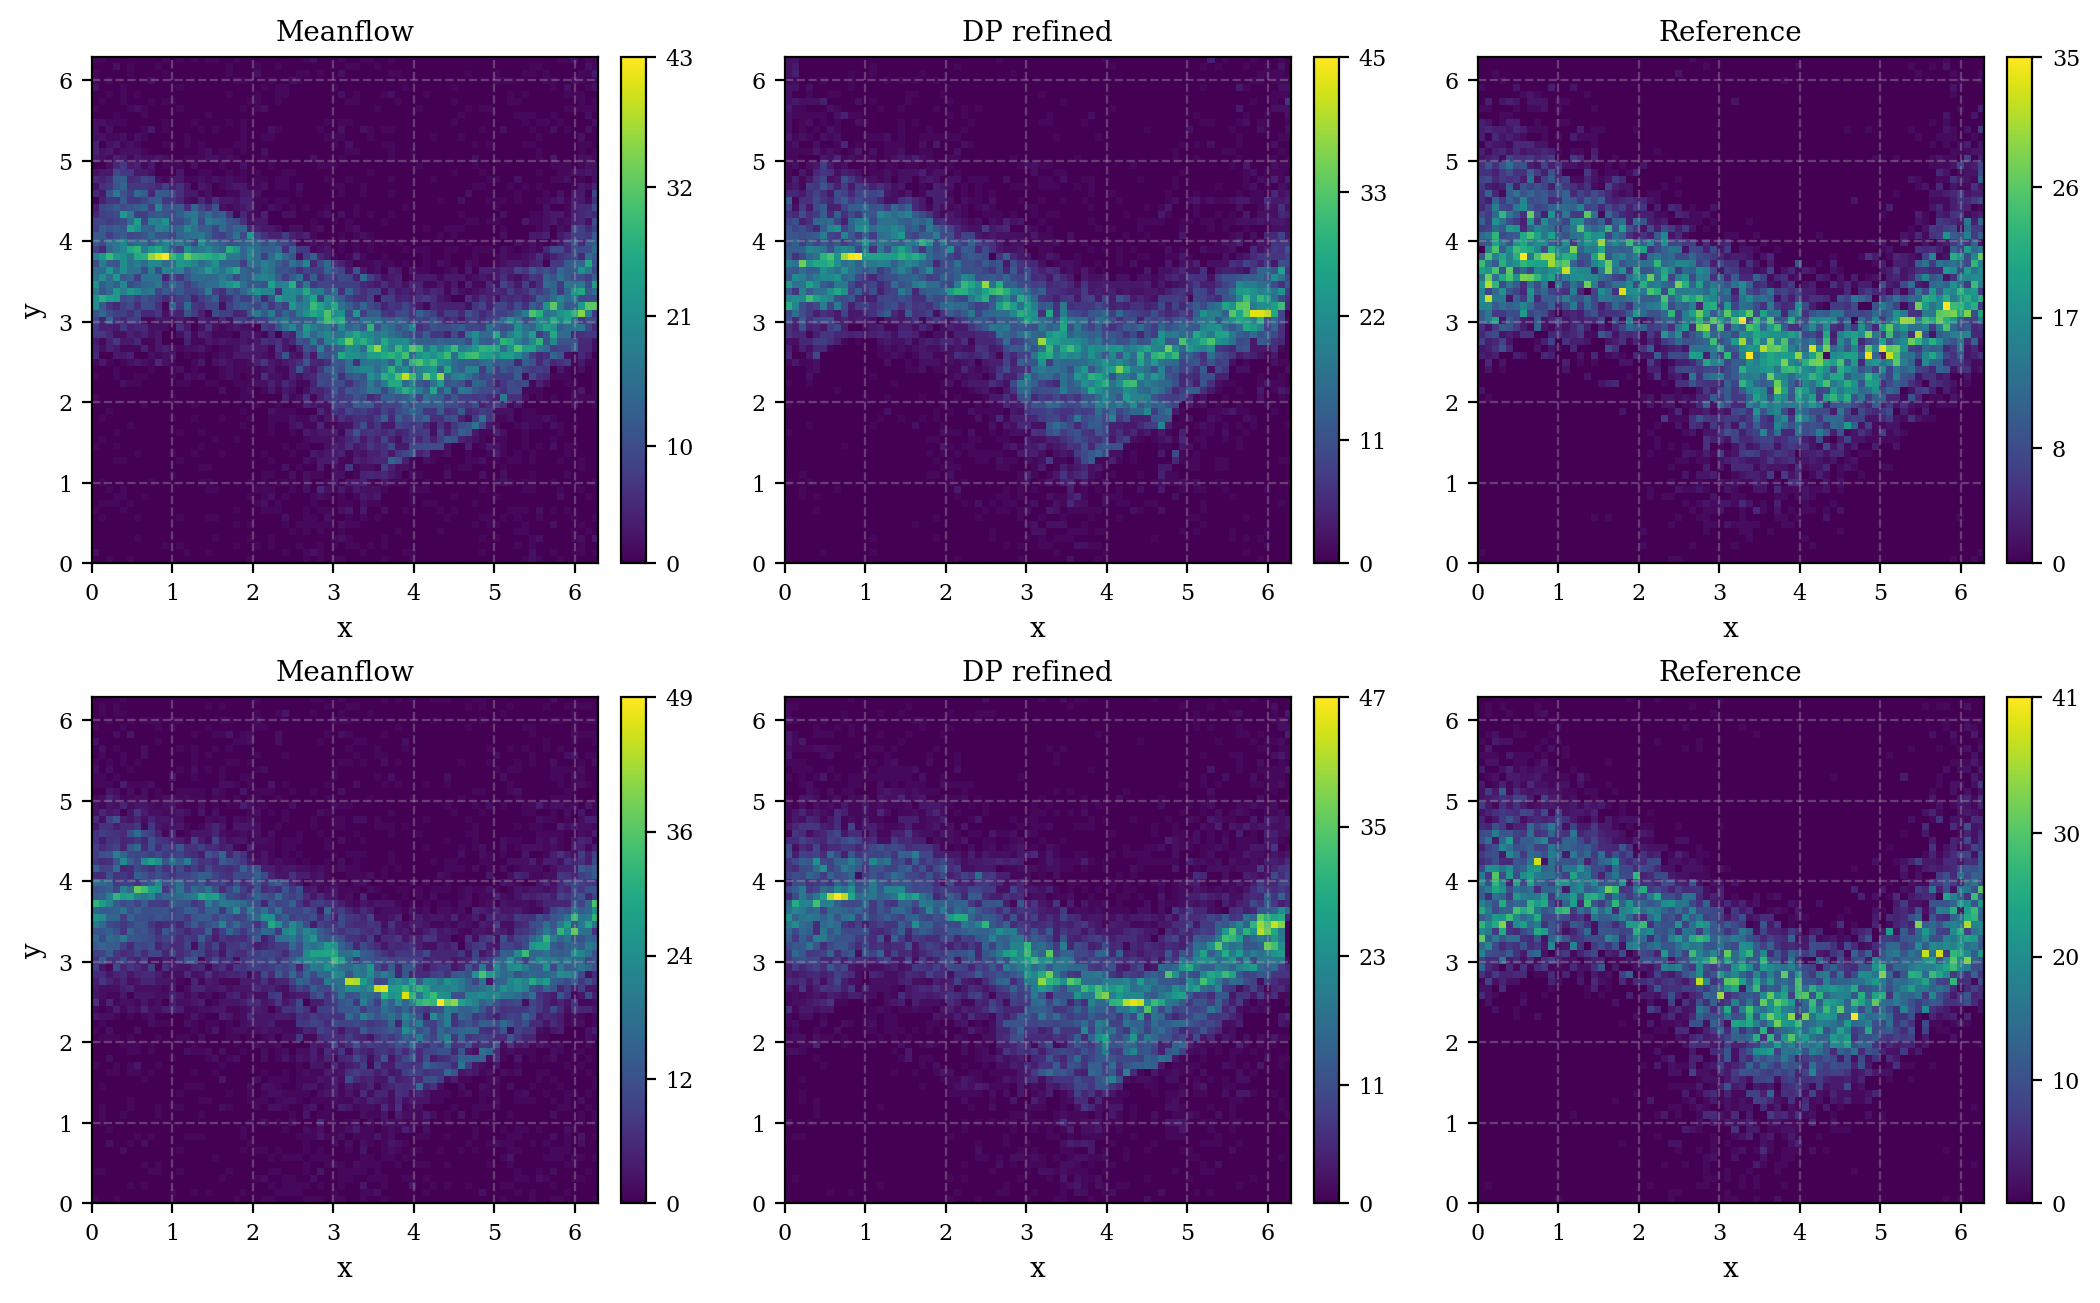
\includegraphics[width=\textwidth]{fig5_invariant_2d.png}
\caption{Empirical invariant measures on \(\mathbb{T}^2\).
Rows are \(\sigma=2^{-3.75}\) (training range) and \(\sigma=2^{-4}\)
(extrapolation). Columns are Meanflow, DP, and the long-horizon
Feynman--Kac reference. Each panel is a \(72\times 72\) count histogram.}
\label{fig:2d-inv}
\end{figure}
\FloatBarrier

\subsubsection{Torus Wasserstein Error}

A uniform cold start remains between \(W_2=1.0538\) and \(1.1718\) on the
eleven-level grid. Meanflow lowers the error to a grid mean of \(0.1434\),
about \(1.9\) times the source-paper Meanflow mean of \(0.0769\). DP has a
grid mean of \(0.1345\) and is below Meanflow on eight of the eleven
levels, including all three extrapolations. At \(-\log_2\sigma=2.00\) the
two values are \(0.0962\) and \(0.1061\). At the end of the training
range, \(-\log_2\sigma=3.75\), Meanflow is \(0.1424\) and DP is
\(0.1368\). At the farthest extrapolation point, \(-\log_2\sigma=4.50\),
Meanflow is \(0.2629\) and DP is \(0.2326\), against \(0.0456\) in the
source paper. Figure~\ref{fig:2d-w2} plots these two columns. The green
line marks the end of the training range. Meanflow error grows past that
boundary. The corrector lowers the error on the finer training levels and
on the extrapolation segment, and does not close the gap to the
source-paper DP column.

\begin{figure}[H]
\centering
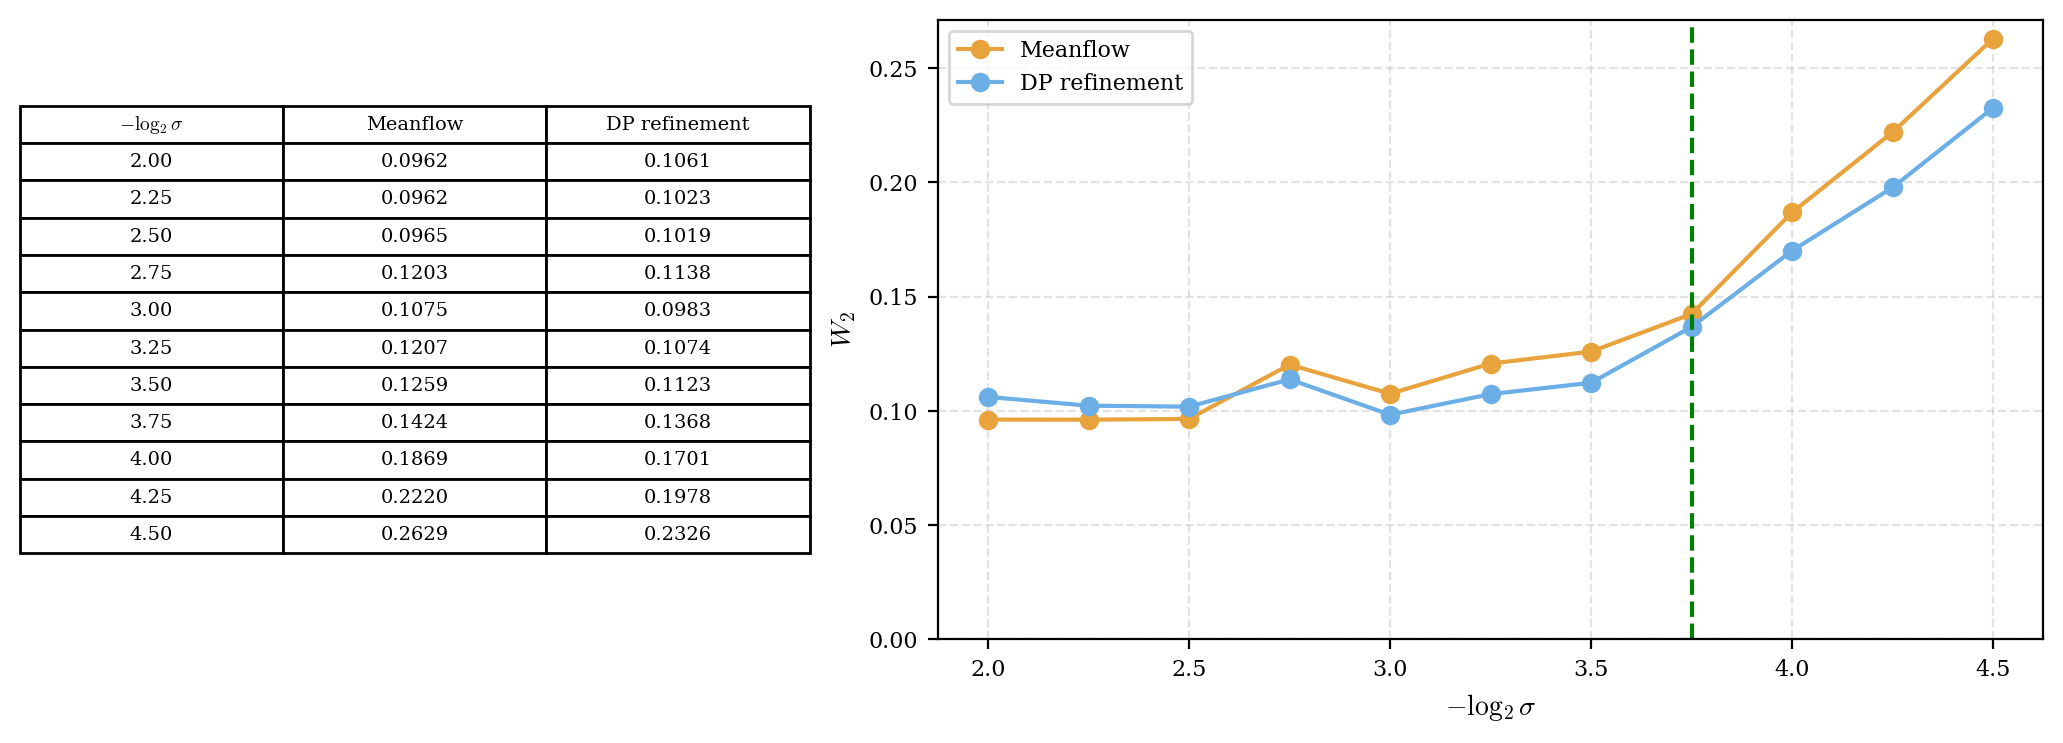
\includegraphics[width=\textwidth]{fig6_w2_2d.png}
\caption{Two-dimensional torus \(W_2\) between the generated cloud and the
Feynman--Kac reference. The left table and the right curves use the same
Meanflow and DP values. The dashed vertical line is
\(-\log_2\sigma=3.75\).}
\label{fig:2d-w2}
\end{figure}
\FloatBarrier

\subsubsection{Eigenvalue estimator}

At \(\sigma=2^{-4.5}\), the long-horizon Feynman--Kac value is
\(\hat c=0.7842\). Figure~\ref{fig:2d-eig} shows that a uniform cold start
begins near \(0.51\) and reaches the reference after about \(10^2\)
generations. The Meanflow warm start is \(0.8180\) at \(T=1\) and
\(0.7841\) at \(T=128\). The DP warm start is \(0.8167\) at \(T=1\) and
\(0.7848\) at \(T=128\). The source paper's DP warm start is \(0.7616\) at
\(T=1\). The log-weight estimator is less sensitive to ridge shape than
the histogram \(W_2\), so a warm start can sit near the Feynman--Kac speed
while the invariant-measure error remains of order \(10^{-1}\).

\begin{figure}[H]
\centering
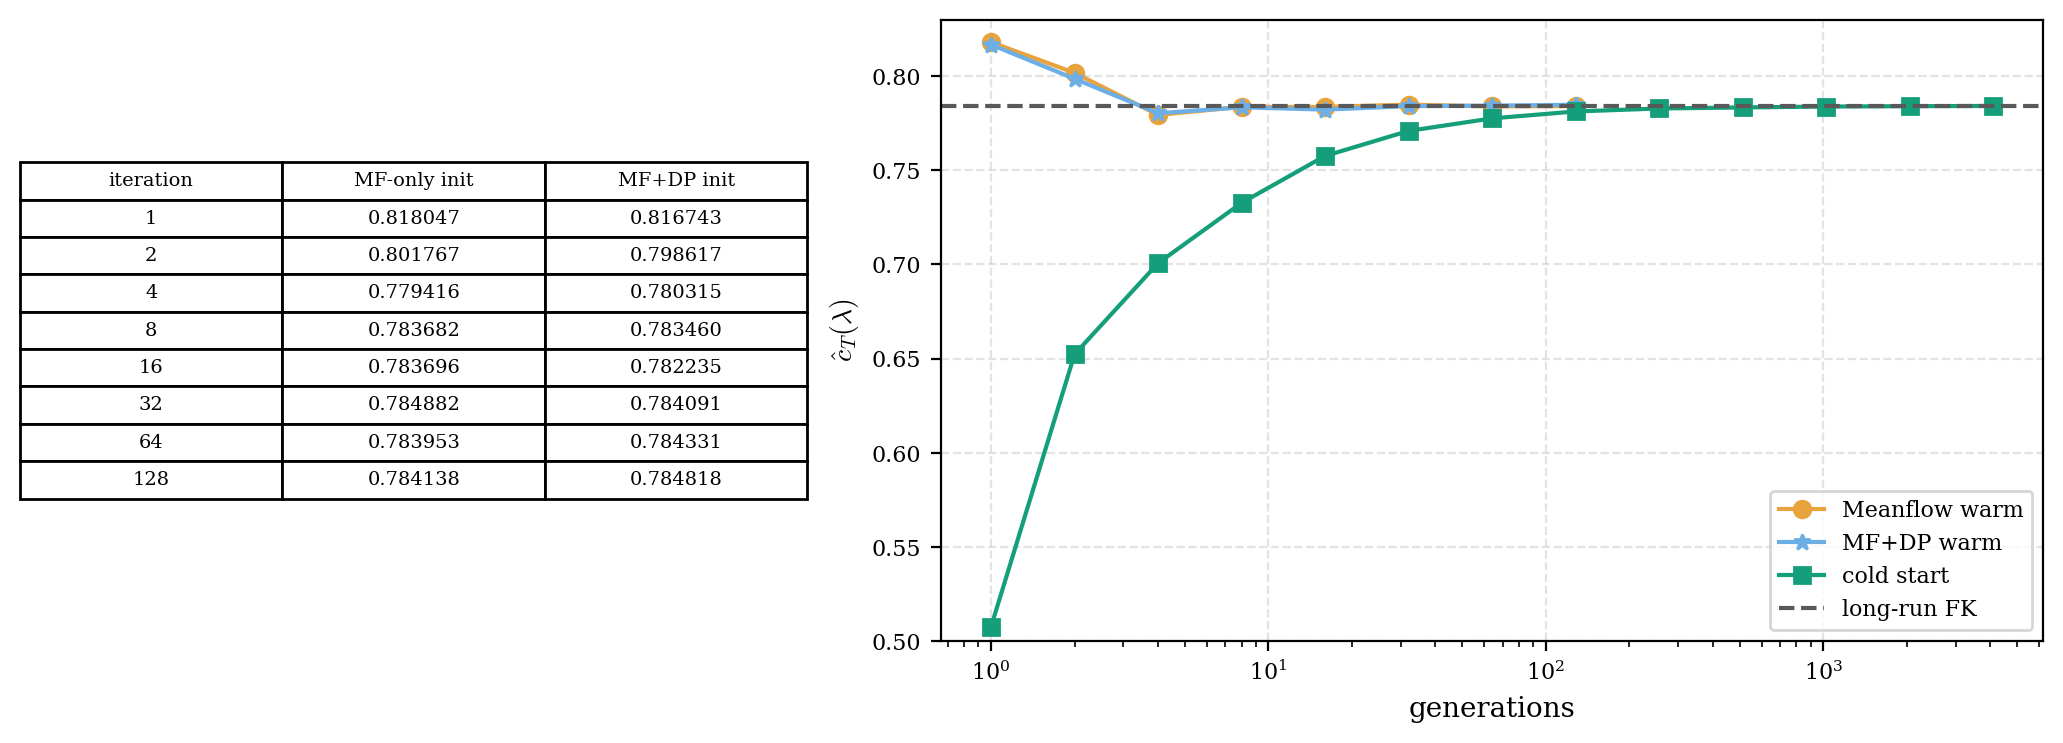
\includegraphics[width=\textwidth]{fig7_eigen_2d.png}
\caption{Two-dimensional front-speed estimator \(\hat c_T(\lambda)\) at
\(\sigma=2^{-4.5}\). The left table lists the two warm starts. The right
panel adds the uniform cold start and the long-horizon Feynman--Kac
reference (dashed). The horizontal axis is logarithmic in the number of
generations.}
\label{fig:2d-eig}
\end{figure}

\FloatBarrier
\clearpage

%----------------------------------------------------------------------
\subsection{3D KPP Front Speed Experiment with Time-Dependent Kolmogorov Flow}
%----------------------------------------------------------------------

\subsubsection{Setting and protocol}

The same KPP equation is posed on \(\mathbb{T}^3=[0,2\pi)^3\), with the
time-dependent Kolmogorov field

\begin{equation}
v(x,t)=\bigl(
\sin(x_3+\sin(2\pi t)),\;
\sin(x_1+\sin(2\pi t)),\;
\sin(x_2+\sin(2\pi t))
\bigr).
\end{equation}

This field is divergence-free for every \(t\). The three-dimensional
reference clouds use the same interacting particle method on
\(\mathbb{T}^3\). The first generation is uniform. The potential is
\(V_\lambda=\kappa\lambda^2+\lambda v\cdot e_1\). Each generation again
covers one forcing period with \(\Delta t=2^{-8}\) and a resample at the
end of the period. After \(T=4096\) generations the
\(M=2\times 10^4\) terminal positions are stored at that \(\sigma\).
Training and evaluation reuse those stored clouds. The remaining
discretization matches the two-dimensional experiment: \(\lambda=2\),
training through \(-\log_2\sigma=3.75\), and evaluation through \(4.50\).
The eigenvalue metric is unchanged. The invariant-measure
error is the \(W_2\) distance of \(x\)-\(z\) projections,

\begin{equation}
\mathcal{E}_{xz}(\sigma)
=W_2\bigl((\Pi_{xz})_{\#}\hat\mu^{(\sigma)},
(\Pi_{xz})_{\#}\hat\nu^{(\sigma)}\bigr),
\end{equation}

where \(\Pi_{xz}(x,y,z)=(x,z)\).

\subsubsection{Projected invariant measure}

At \(\sigma=2^{-4.5}\), the Feynman--Kac cloud is anisotropic across the
three coordinate planes. Mass concentrates at larger \(z\) in the
\(x\)-\(z\) and \(y\)-\(z\) views, and the \(y\)-\(z\) plane shows a curved
ridge. This structure is consistent with a potential \(V_\lambda\) that
depends on \(x_3\) through the first velocity component.
Figure~\ref{fig:3d-inv} compares the three planes for the reference,
Meanflow, and DP. Meanflow recovers the high-\(z\) concentration and the
main anisotropy of each plane, with a noisier footprint than the
reference. DP tightens those planes relative to Meanflow. The \(x\)-\(y\)
view recovers the two opposing chevrons of the Feynman--Kac cloud, and
the \(y\)-\(z\) ridge is thinner than the Meanflow band. Both generated
clouds remain grainier than the reference. The \(x\)-\(z\) plane is the
one used for the \(W_2\) numbers below.

\begin{figure}[H]
\centering
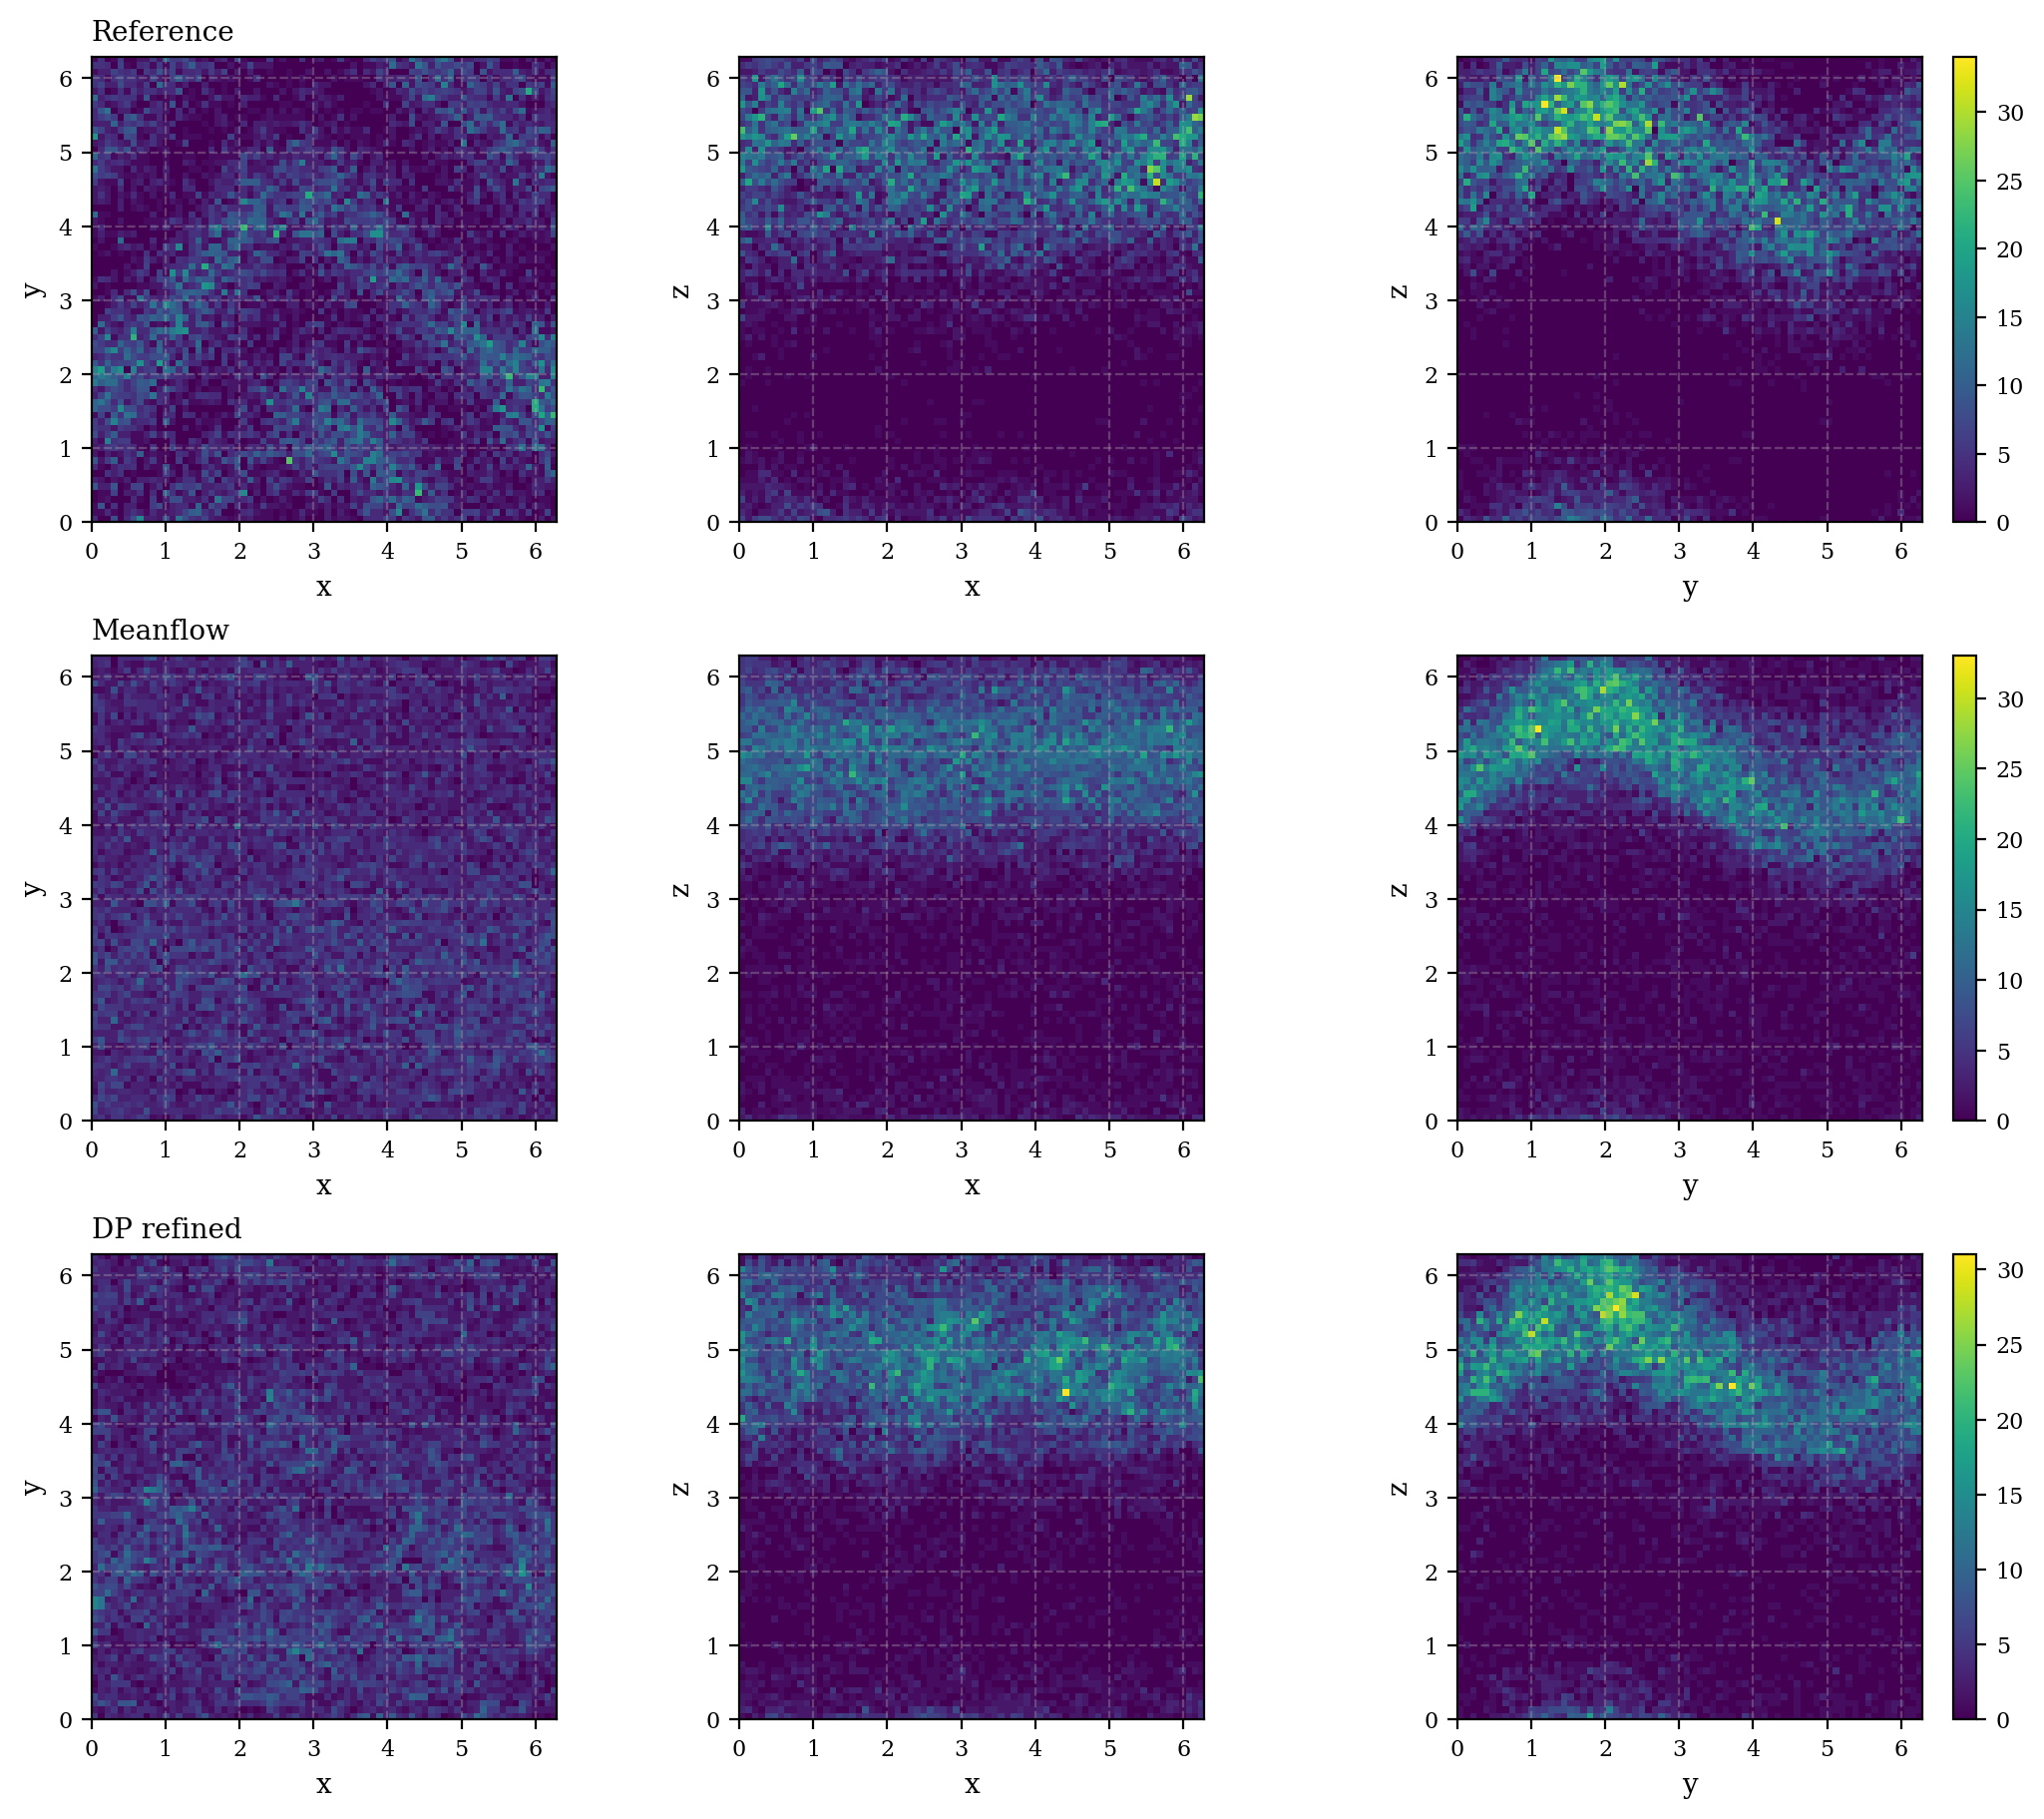
\includegraphics[width=0.88\textwidth]{fig8_projections_3d.png}
\caption{Three-dimensional invariant-measure projections at
\(\sigma=2^{-4.5}\). Rows are the Feynman--Kac reference, Meanflow, and
DP. Columns are the \(x\)-\(y\), \(x\)-\(z\), and \(y\)-\(z\) planes.
Each row shares a colorbar.}
\label{fig:3d-inv}
\end{figure}
\FloatBarrier

\subsubsection{Projected Wasserstein Error}

The uniform cold start remains between \(0.8895\) and \(0.9600\) on the
grid. Meanflow lowers the projected error to a mean of \(0.1293\), next
to the source-paper Meanflow mean of \(0.1312\). DP has a grid mean of
\(0.1065\) and a minimum of \(0.0920\) at \(-\log_2\sigma=2.75\). The
source-paper DP mean is \(0.0294\). At \(-\log_2\sigma=4.50\), Meanflow
is \(0.1582\) and DP is \(0.1366\). Figure~\ref{fig:3d-w2} plots these
two columns. DP is larger than Meanflow only at the coarsest training
level and smaller at the remaining ten, including the farthest
extrapolation point.

\begin{figure}[H]
\centering
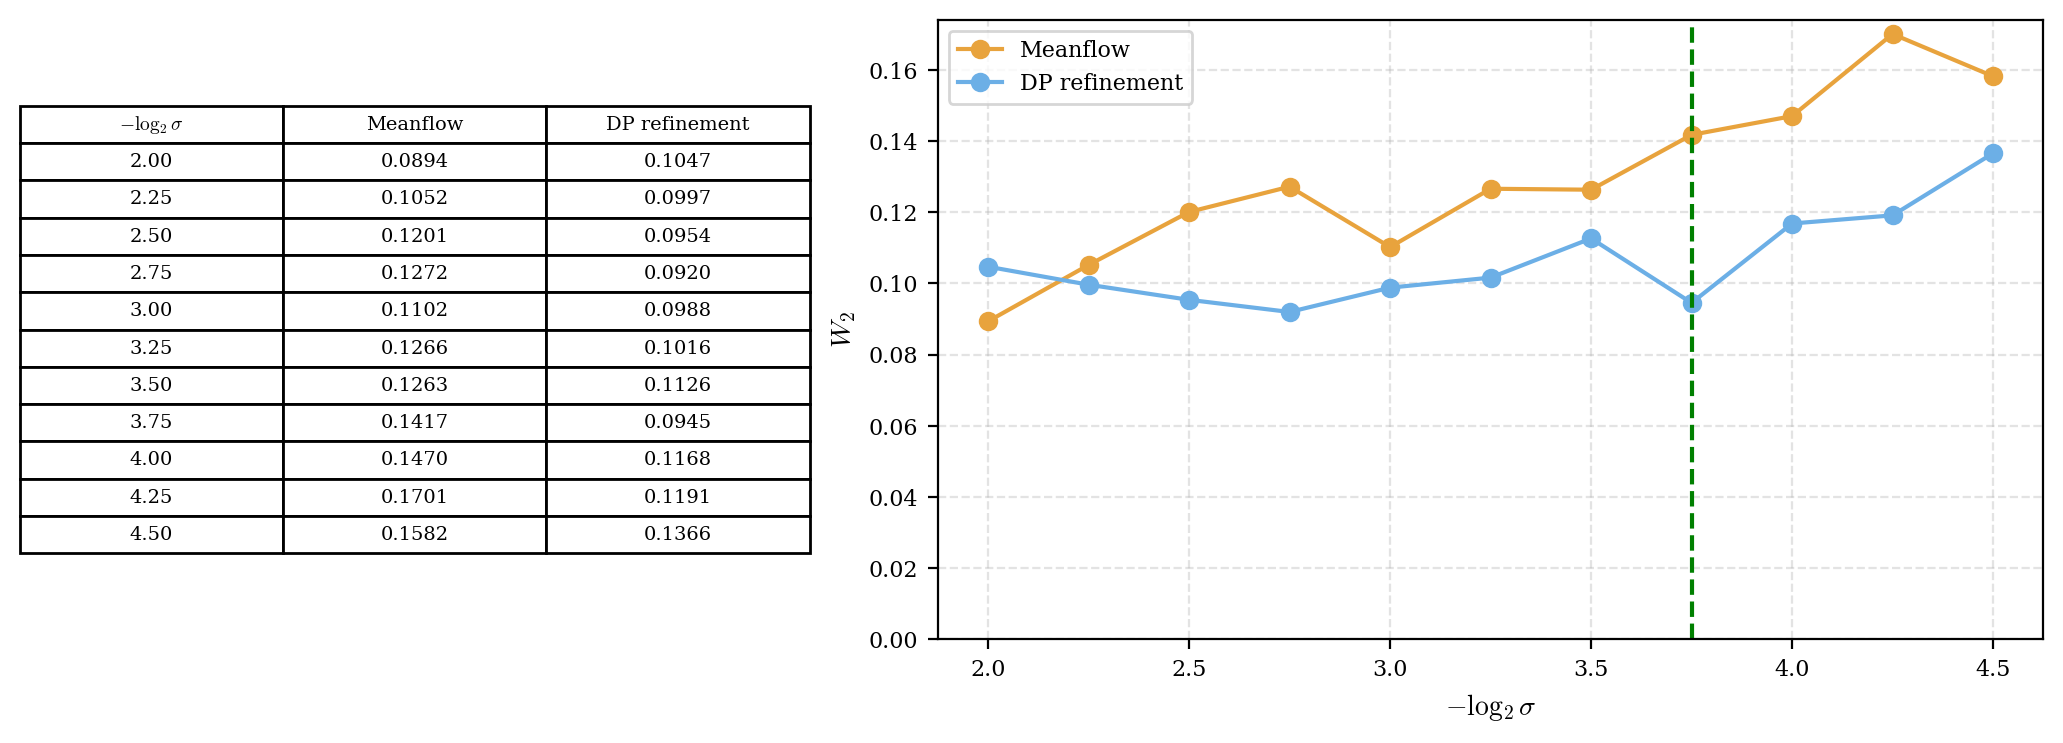
\includegraphics[width=\textwidth]{fig9_w2_3d.png}
\caption{Projected \(x\)-\(z\) \(W_2\) on \(\mathbb{T}^3\). The left table
and the right curves use the same Meanflow and DP values. The dashed
vertical line is \(-\log_2\sigma=3.75\).}
\label{fig:3d-w2}
\end{figure}
\FloatBarrier

\subsubsection{Eigenvalue estimator}

At \(\sigma=2^{-4.5}\), the long-horizon Feynman--Kac value is
\(0.6147\). Figure~\ref{fig:3d-eig} shows a cold start near \(0.36\) that
reaches the reference by about \(10^2\) generations. Meanflow is
\(0.6148\) at \(T=1\) and \(0.6131\) at \(T=128\). DP is \(0.6171\) at
\(T=1\) and \(0.6142\) at \(T=128\). The source paper's DP warm start is
\(0.6135\) at \(T=1\). As in two dimensions, the eigenvalue can sit near
the Feynman--Kac limit while the projected \(W_2\) remains of order
\(10^{-1}\). The reproduced Meanflow projected \(W_2\) sits near the
source-paper Meanflow column. The DP refinement does not reach the
source-paper DP table.

\begin{figure}[H]
\centering
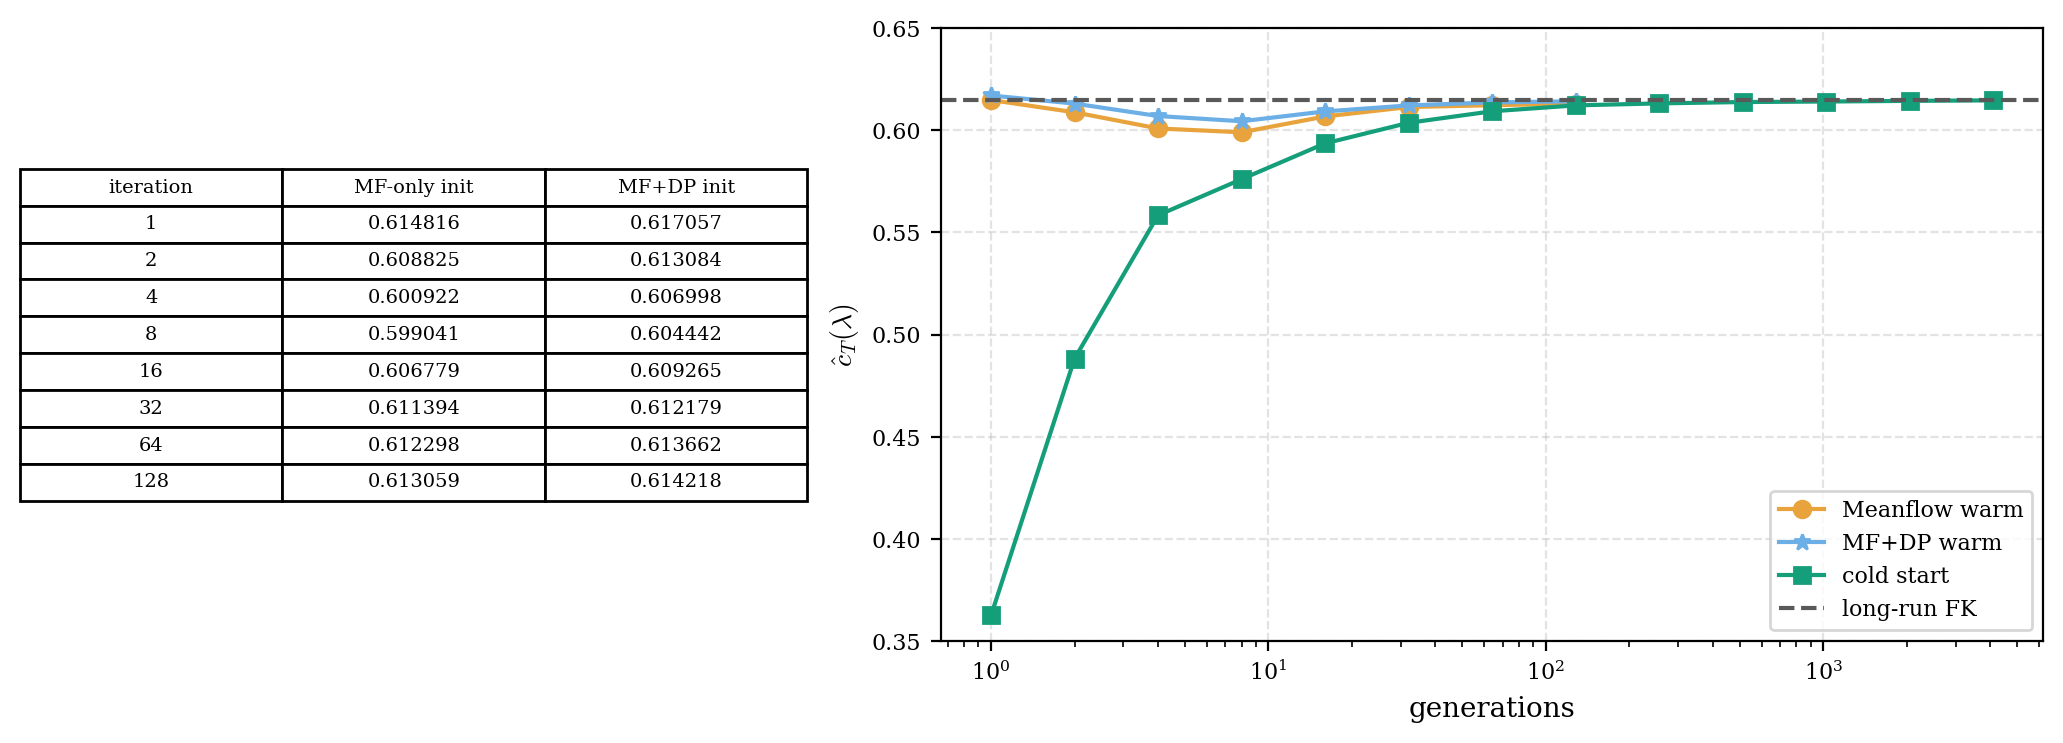
\includegraphics[width=\textwidth]{fig10_eigen_3d.png}
\caption{Three-dimensional front-speed estimator \(\hat c_T(\lambda)\) at
\(\sigma=2^{-4.5}\). The left table lists the two warm starts. The right
panel adds the uniform cold start and the long-horizon Feynman--Kac
reference (dashed). The horizontal axis is logarithmic in the number of
generations.}
\label{fig:3d-eig}
\end{figure}

\begin{thebibliography}{9}
\bibitem{wang2022deepparticle}
Z.~Wang, J.~Xin, and Z.~Zhang.
\newblock DeepParticle: learning invariant measure by a deep neural network
minimizing Wasserstein distance on data generated from an interacting
particle method.
\newblock \emph{J.\ Comput.\ Phys.} 464 (2022) 111309.
\end{thebibliography}

\end{document}
